\documentclass[10pt]{standalone}
\usepackage{commands}

\begin{document}
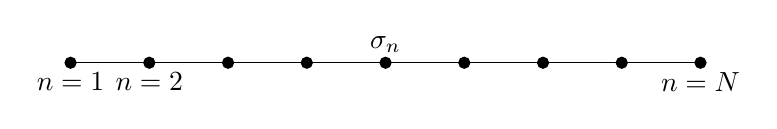
\begin{tikzpicture}
    \draw[] (0, 0) -- (8, 0);
    \foreach \i in {0,...,8} {
        \filldraw (\i, 0) circle (2pt);
    };
    \node[below] at (0, 0) {$n=1$};
    \node[below] at (1, 0) {$n=2$};
    \node[below] at (8, 0) {$n = N$};
    \node[above] at (4, 0) {$\sigma_n$};
\end{tikzpicture}
\end{document}